\documentclass[11pt]{scrartcl}
\usepackage{graphicx}
\graphicspath{{./}}
\usepackage[sexy]{evan}
\usepackage[normalem]{ulem}
\usepackage{hyperref}
\usepackage{mathtools}
\hypersetup{
    colorlinks=true,
    linkcolor=blue,
    filecolor=magenta,      
    urlcolor=cyan,
    pdfpagemode=FullScreen,
    }

\renewcommand{\dangle}{\measuredangle}

\renewcommand{\baselinestretch}{1.5}

\addtolength{\oddsidemargin}{-0.4in}
\addtolength{\evensidemargin}{-0.4in}
\addtolength{\textwidth}{0.8in}
% \addtolength{\topmargin}{-0.2in}
% \addtolength{\textheight}{1in} 


\setlength{\parindent}{0pt}

\usepackage{pgfplots}
\pgfplotsset{compat=1.15}
\usepackage{mathrsfs}
\usetikzlibrary{arrows}

\title{Soal Try Out OSN SD}
\author{Azzam (IG: haxuv.world)}
\date{Selasa, 19 Februari 2024}

\begin{document}
\maketitle
\textbf{Aturan umum:}
\begin{itemize}
    \item \textbf{Soal bertipe ISIAN SINGKAT}. Jawab dengan hasil akhirnya saja
    \item Setiap soal bernilai 2,5 jika benar dan 0 jika salah atau kosong.
\end{itemize}

\section{Soal}
\begin{enumerate}
\item Nilai dari $1+3+5+7+\ldots+19$ adalah \dots
\item Nilai dari $9 + 2 \times \frac{22}{4} – \frac{8}{8}$ adalah....
\item Selisih nilai antara angka $5$ dan angka $8$ dari bilangan $75289$ adalah...
\item Perbandingan jumlah anak laki-laki dan perempuan dalam lomba olympiade MIPA di Kabupaten Luwu Timur adalah $5:3$ jika terdapat $20$ anak laki-laki lebih banyak dari perempuan. Jumlah anak perempuan dalam olimpiade MIPA tersebut adalah....
\item Jumlah $3$ bilangan yang berurutan adalah $294$, bilangan yang terbesar dari bilangan itu adalah...
\item $12$ baju yang sedang dijemur disebuah halaman rumah membutuhkan waktu $6$ jam agar kering. Jika dijemur $4$ buah baju berapa waktu yang dibutuhkan agar keempat baju tersebut kering (dengan panas yang sama)?
\item Arnol membeli sebuah pulpen dengan harga Rp $5.500,-$ dan sebuah buku cetak yang harganya tiga kali lipat dari harga pulpen. Berapa total yang harus dibayar oleh Arnol.
\item Sekarang hari sabtu (tanggal $6$ Desember $2008$), jatuh pada hari apakah $100$ hari yang akan datang?
\item Selisih antara $40\%$ dari Rp $60.000$ dan $25\%$ dari Rp.$40.000$ adalah...

\item Hasan bersepeda dari Wawondula ke Sorowako dengan kecepatan $12$ km/jam, dan ia menempuh dalam waktu $2$ jam. Hitunglah jarak Wawondula ke Sorowako!

\item Dalam suatu acara pesta perkawinan, disusun kursi dengan baris paling depan terdiri dari $12$ buah, baris kedua $14$ buah, baris ketiga $16$ buah, dan seterusnya. Hitunglah banyaknya kursi pada baris ke-$20$.
\item Berapa banyaknya bilangan bulat yang mempunyai angka $5$ antara bilangan $1$ sampai dengan $100$.
\item Sebuah ruangan berbentuk persegipanjang dengan panjang $10$ m dan lebar $6$ m, akan dipasangi ubin dengan ukuran $40$ cm x $40$ cm. berapa banyak ubin yang dibutuhkan?
\item Seekor keong berada di dasar sumur. Pada waktu sepuluh menit pertama, keong memanjat $2 \frac{2}{3}$ m , pada $10$ menit ke dua, ia memanjat $1 \frac{4}{3}$ m. Setelah $20$ menit, berapa jauh keong tersebut dari dasar sumur?
\item Andi memberikan $50\%$ kelerengnya untuk Wawan dan $25\%$ dari sisanya itu diberikan Rudy. Dia masih mempunyai $90$ kelereng yang sisa. Berapa jumlah kelereng mula-mula?
\item Bilangan decimal $0,135135....$ Dapat dinyatakan dalam bentuk $\frac{a}{b}$ , maka nilai $a+b$ adalah...
\item Diberikan sebuah bilangan yang merupakan hasil perkalian $4$, bilangan itu antara $6$ dan $15$. bilangan itu juga merupakan factor dari $16$. bilangan berapakah itu?
\item Keliling sebuah persegi adalah $48$, maka luas persegi adalah...
\item Tentukan angka satuan dari $7^{125}$.
\item Bilangan $5$ angka $6A47A$ habis dibagi $8$. Nilai $A$ adalah...
\item Sebuah buku resep makanan tergeletak dalam keadaan terbuka diatas meja.
jika bilangan yang menunjukkan kedua halaman yang terbuka itu dikalikan, hasilnya adalah $1190$. Pada halaman berapakah buku tersebut terbuka.

\item Dalam suatu gedung terdapat $20$ kursi pada baris pertama dan setiap baris berikutnya memuat $2$ kursi lebih banyak. Banyaknya kursi pada baris ke $20$ adalah...
\item Jumlah $7$ bilangan berurutan adalah $91$. Tentukan bilangan terkecil dari urutan bilangan itu.
\item Jika bangunan dibawah ini memiliki keliling $36$ cm, berapa keliling masing- masing segitiga kecil? (bangun segitiga sama sisi)
\begin{figure}[h]
    \centering
    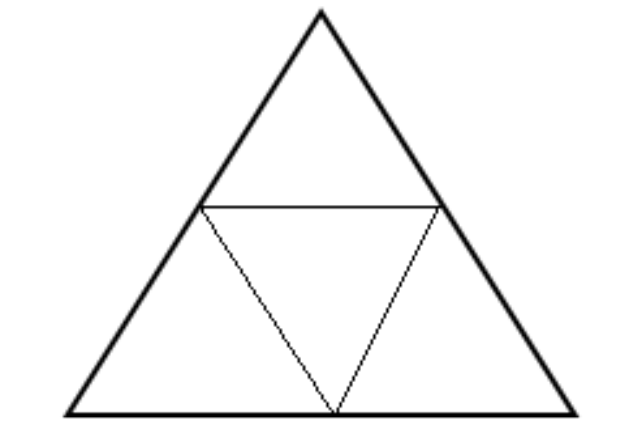
\includegraphics[scale=0.3]{Test For Pelatihan/TryOut OSN SD/segitigaSamaSisi.png}
    \label{fig:enter-label}
\end{figure}
\item Luas sebuah bujur sangkar sama luasnya dengan persegipanjang. Jika keliling bujur sangkar $24$ cm, dan lebar persegipanjang $4$ cm. Hitunglah berapa cm ukuran panjang persegipanjang?
\item Jika luas persegipanjang $ABCD$ adalah $320$ cm$^2$. Maka luas daerah yang diarsir pada gambar adalah...
\begin{figure}[h]
    \centering
    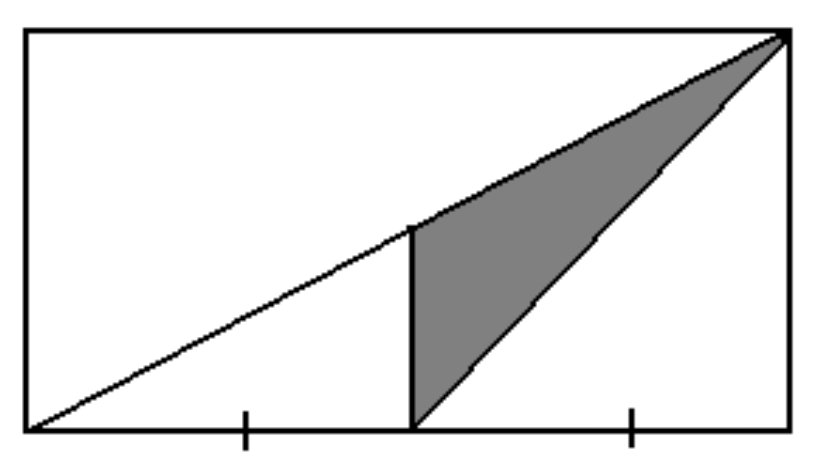
\includegraphics[scale=0.3]{Test For Pelatihan/TryOut OSN SD/persegiPanjangDiarsir.png}
    \label{fig:enter-label}
\end{figure}
\item $40\%$ dari kursi di sebuah pesawat adalah kursi kelas A, sisanya adalah kursi kelas B dan kelas ekonomi. Perbandingan jumlah kursi kelas B dan ekonomi adalah $5:7$. Jika jumlah kursi kelas ekonomi $80$ lebih banyak dari kursi kelas B, berapa jumlah seluruh kursi dalam pesawat?
\item Anita baru saja membeli sebuah buku. Setiap harinya, ia membaca buku itu dalam jumlah halaman yang selalu sama. Setelah $8$ hari, ia telah membaca $\frac{3}{4}$ dari isi buku tersebut. $4$ hari kemudian tinggal $100$ halaman buku yang belum dibacanya. Berapa jumlah total halaman buku tersebut?
\item Sebuah kertas berbentuk persegi dilipat dua dan kemudian di potong menjadi dua persegipanjang sepanjang lipatan tadi. Keliling tiap persegi panjang adalah $18$ cm. Berapa keliling persegi mula-mula?
\begin{figure}[h]
    \centering
    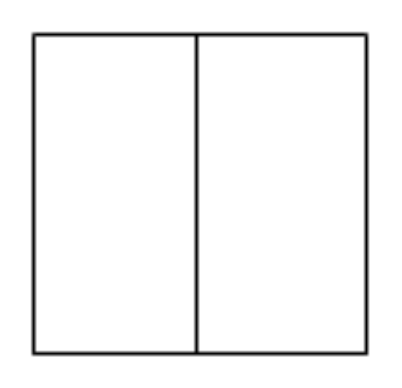
\includegraphics[scale=0.3]{Test For Pelatihan/TryOut OSN SD/persegiDibelah.png}
\label{fig:enter-label}
\end{figure}
\item Usia rata-rata dari siswa di kelasnya Andi adalah 12 tahun. Usia rata-rata siswa dikelas Awal adalah 15 tahun. Jika terdapat 40 siswa di kelas Andi dan 42 siswa dikelas Awal, hitunglah usia rata-rata di kedua kelas tersebut?

\item The average of $x$ and $y$ is $19$. The average of $a$, $b$ and $c$ is $14$. Find the average of $x$, $y$, $a$, $b$ and $c$. 

\item Find the units digit for the following sum: $23^{2011} + 37^{2011}  + 64^{2011}  + 88^{2011} $. 

\item There are two positive integers, neither of which has a digit equal to $0$, whose product is $8000$. Find the sum of these two positive integers. 

\item The diagram shows two semicircles with $AB$ touching the smaller semicircle and parallel to $CD$. Given $AB = 14$ cm, find the area of the shaded region, in cm$^2$. 
\begin{figure}[h]
    \centering
    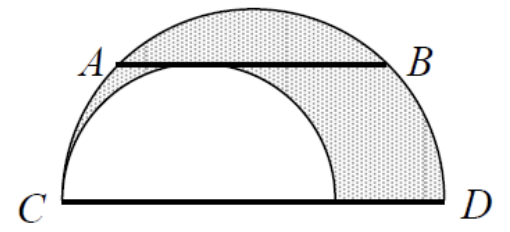
\includegraphics[scale=0.5]{Test For Pelatihan/TryOut OSN SD/semiCircle.png}
    \label{fig:enter-label}
\end{figure}

\item In the diagram shown, find the measure of $\angle a +\angle b +\angle c +\angle d +\angle e$.
\begin{figure}[h]
    \centering
    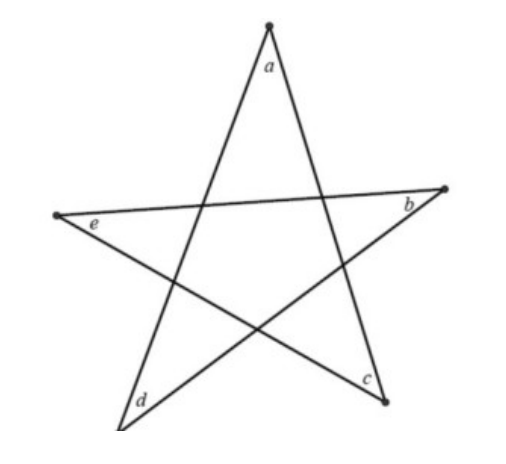
\includegraphics[scale=0.7]{Test For Pelatihan/TryOut OSN SD/star.png}
    \label{fig:enter-label}
\end{figure}

\item Let : $A = 202320232023 \times 2024202420242024$ and $B = 202420242024 \times 2023202320232023$. Find $A - B$.

\item Given that $1^2+2^2+3^2+\ldots+n^2=\dfrac{n(n+1)(2n+1)}{6}$. Find The Value of $1^2+3^2+5^2+7^2+\ldots+99^2$

\item Arrange the numbers $2^{847}$, $3^{539}$ ,$5^{363}$ , $7^{308}$ and $11^{242}$ from the largest to the smallest.

\item A sequence of digits is formed by writing the digits from the natural numbers in the order that they appear. The sequence starts : $123456789101112 \ldots$\\
What is the $2024$th digit in the sequence?

\item The fraction $\dfrac{2024}{7000}$ is written as a decimal. What digit is in the $2024$th place? (In the decimal $0,23456$ the digit $4$ is in the $3$rd place.)
\end{enumerate}




\end{document}
